\section{Experimental setup}
\label{sec:experiments}

\subsection{Forward modeling}
\label{subsec:synthetic_data}

Synthetic first-arrival times are generated independently of EMTomo using PyKonal 0.4.1 \parencite{white2020pykonal}. The generator solves the Cartesian eikonal equation from the true event coordinates on a refined nodal grid, initializes off-grid sources with local straight-segment slowness integrals, and samples receivers by interpolating the regular factor $T(\mathbf{x})/\|\mathbf{x}-\mathbf{h}\|$. This differs from EMTomo's station-centered \texttt{scikit-fmm} fields, homogeneous source-sphere initialization, and direct interpolation of travel times. Separate solvers, grids, and source treatments reduce numerical inverse crime; both still approximate the same isotropic first-arrival problem, so this is not a test against independent wave physics.

Before referencing each event to its earliest observed arrival, we add independent relative and absolute Gaussian errors,
\begin{equation}
t^{\mathrm{noisy}}_{en}=T^{\mathrm{true}}_{en}
+0.01T^{\mathrm{true}}_{en}Z^{(1)}_{en}+\sigma_a Z^{(2)}_{en},
\qquad Z^{(1)}_{en},Z^{(2)}_{en}\sim\mathcal{N}(0,1),
\end{equation}
where $\sigma_a$ is the absolute timing-noise standard deviation. Both methods use the same noisy picks; inter-event differential times for tomoDD are formed from these picks without additional waveform cross-correlation observations. Initial hypocenters for tomoDD are obtained by adding independent zero-mean Gaussian perturbations to each true coordinate, with out-of-domain positions rejection-resampled. EMTomo does not require an initial hypocenter catalog.

\subsection{Evaluation}
\label{subsec:metrics}

\paragraph{Velocity fields.}
We evaluate the native reconstructed fields at the same physical points $\{\mathbf{x}_q\}_{q=1}^Q$, without converting one method to the other's parameterization. EMTomo is piecewise constant; tomoDD is evaluated by its native trilinear velocity interpolation, including the fixed exterior nodes. We assess whole-volume velocity accuracy using the root-mean-square error,
\begin{equation}
\mathrm{RMSE}_v=\sqrt{\frac{1}{Q}\sum_q[\widehat v(\mathbf{x}_q)-v^{\mathrm{true}}(\mathbf{x}_q)]^2}.
\label{eq:velocity_metrics}
\end{equation}
For each representation, a truth-only oracle fits velocity values to the known field, without using arrivals or estimating hypocenters. For constant cells, the volume squared-error optimum is the arithmetic mean of true velocity within each cell, \emph{not} the inverse of mean slowness. For tomoDD we use the saved least-squares trilinear truth fit with the same free nodes and fixed exterior values as the inversion. These references quantify representational error, not the resolution attainable from the available rays, and are distinct from an inversion with fixed true hypocenters. A whole-volume oracle is not a lower bound for every regional RMSE, and the difference between reconstruction and oracle RMSE is not an additive decomposition of inversion error.

The checkerboard truth is exactly representable by EMTomo's aligned constant cells, so its oracle is the true field. This is \emph{not} true for the layered sphere models on the coarser inversion grid: they require a separate cell-mean oracle. Because the two layered experiments share the same truth and grids, they share both representation oracles and initial native fields.

\paragraph{Hypocenters.}
We assess hypocenter accuracy using the 90th percentile of the three-dimensional location errors $d_e=\|\widehat{\mathbf{h}}_e-\mathbf{h}^{\mathrm{true}}_e\|$, in meters, with all events weighted equally. For soft EMTomo, we use the hypothesis with the largest weight as the point estimate.

\paragraph{Spherical anomalies.}
For each of the six spherical anomalies, we additionally evaluate velocity RMSE over its known nonzero support $S_k$:
\begin{equation}
\mathrm{RMSE}_{v,k}=\sqrt{\frac{1}{Q_k}\sum_{\mathbf{x}_q\in S_k}
[\widehat v(\mathbf{x}_q)-v^{\mathrm{true}}(\mathbf{x}_q)]^2},
\qquad k=1,\ldots,6,
\label{eq:sphere_rmse}
\end{equation}
where $Q_k$ is the number of evaluation points in $S_k$. Thus each reconstruction is characterized by one whole-volume RMSE and six individual anomaly RMSE values. The anomaly supports are defined by the true model, without segmenting the reconstructed field.


\section{Results}
\label{sec:results}

\subsection{Checkerboard test}
\label{subsec:checkerboard_results}

The checkerboard models occupy a $24\times12\times12$~km domain. Alternating cubes have velocities 4.75 and 5.25~km/s and sides 6, 4, or 3~km, corresponding to $n_x=4,6,8$ cubes along the $X$ axis. All three models share 1200 events and 98 surface stations (Figure~\ref{fig:checkerboard_geometry_current}). Both methods start from a homogeneous 5~km/s velocity model and use 1-km velocity parameterizations. Arrival-time noise combines 1\% relative errors with $\sigma_a=0.01$~s; the initial tomoDD hypocenters are perturbed with a 1-km standard deviation per coordinate. EMTomo uses 12 hard-assignment updates, selecting one of 15 candidates, with $\lambda=1$ and coverage-damping power zero; tomoDD uses three joint iterations.

\begin{figure}[!htb]
\centering
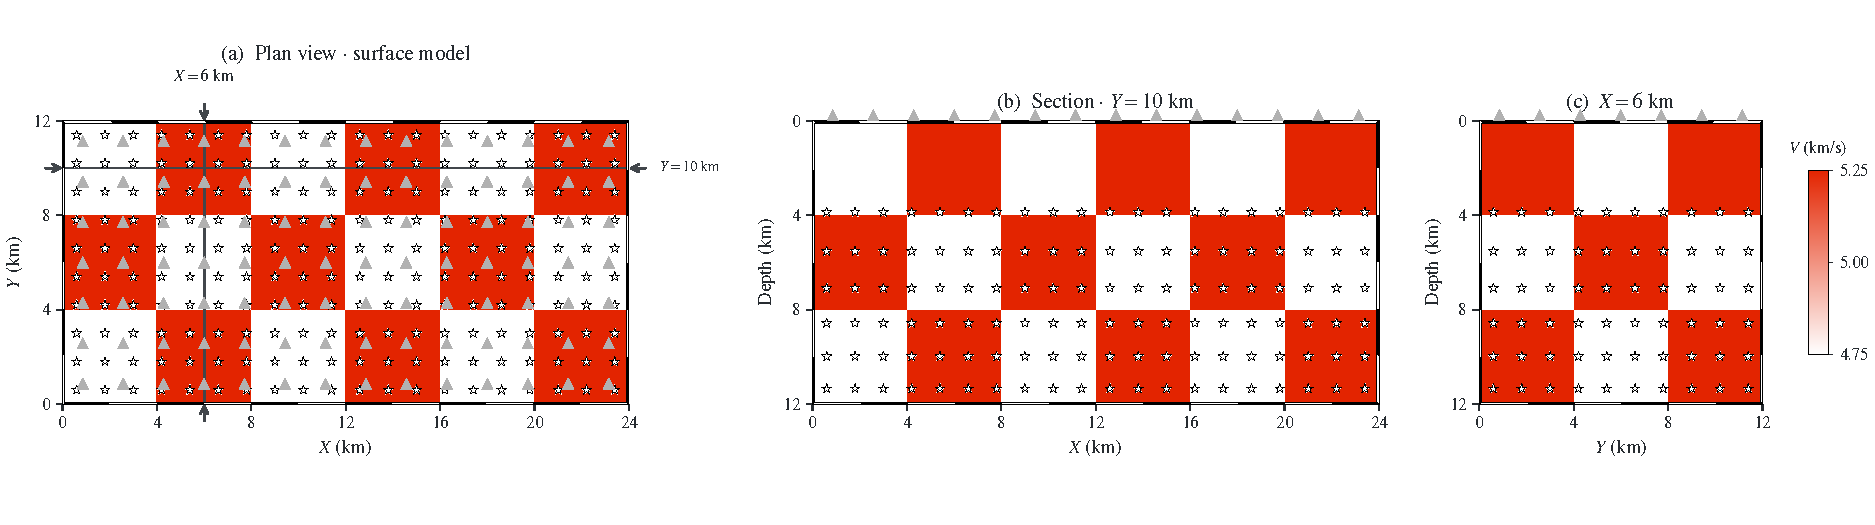
\includegraphics[width=\textwidth]{figures/checkerboard_nx6_geometry.pdf}
\begin{singlespace}
\caption{Checkerboard model and acquisition geometry for $n_x=6$. (a) Surface velocity field and plan-view projections of stations (grey triangles) and events (white stars). (b,c) Vertical sections at $Y=10$~km and $X=6$~km, with stations and events projected onto each plane; coincident projections are drawn once. Depth is positive downward.}
\label{fig:checkerboard_geometry_current}
\end{singlespace}
\end{figure}

Figure~\ref{fig:checkerboard_comparison_current} compares the reconstructed velocity fields with the truth and the trilinear representation oracle. Table~\ref{tab:checkerboard_velocity} reports whole-volume RMSE, evaluated on a common uniform grid of voxel centers with 31.25-m spacing.

\begin{table}[!htb]
\centering
\begin{singlespace}
\caption{Checkerboard whole-volume velocity RMSE (m/s). The common homogeneous initial model has RMSE 250~m/s; the EMTomo representation oracle has zero error. The saved trilinear oracle is evaluated on the same grid, without refitting.}
\label{tab:checkerboard_velocity}
\begin{tabular}{rrrrr}
\toprule
$n_x$ & Cube side (km) & EMTomo & tomoDD & Trilinear oracle \\
\midrule
4 & 6 & 175.3 & 199.2 & 76.2 \\
6 & 4 & 155.7 & 215.1 & 98.8 \\
8 & 3 & 150.8 & 221.2 & 117.4 \\
\bottomrule
\end{tabular}
\end{singlespace}
\end{table}

\begin{figure}[!htb]
\centering
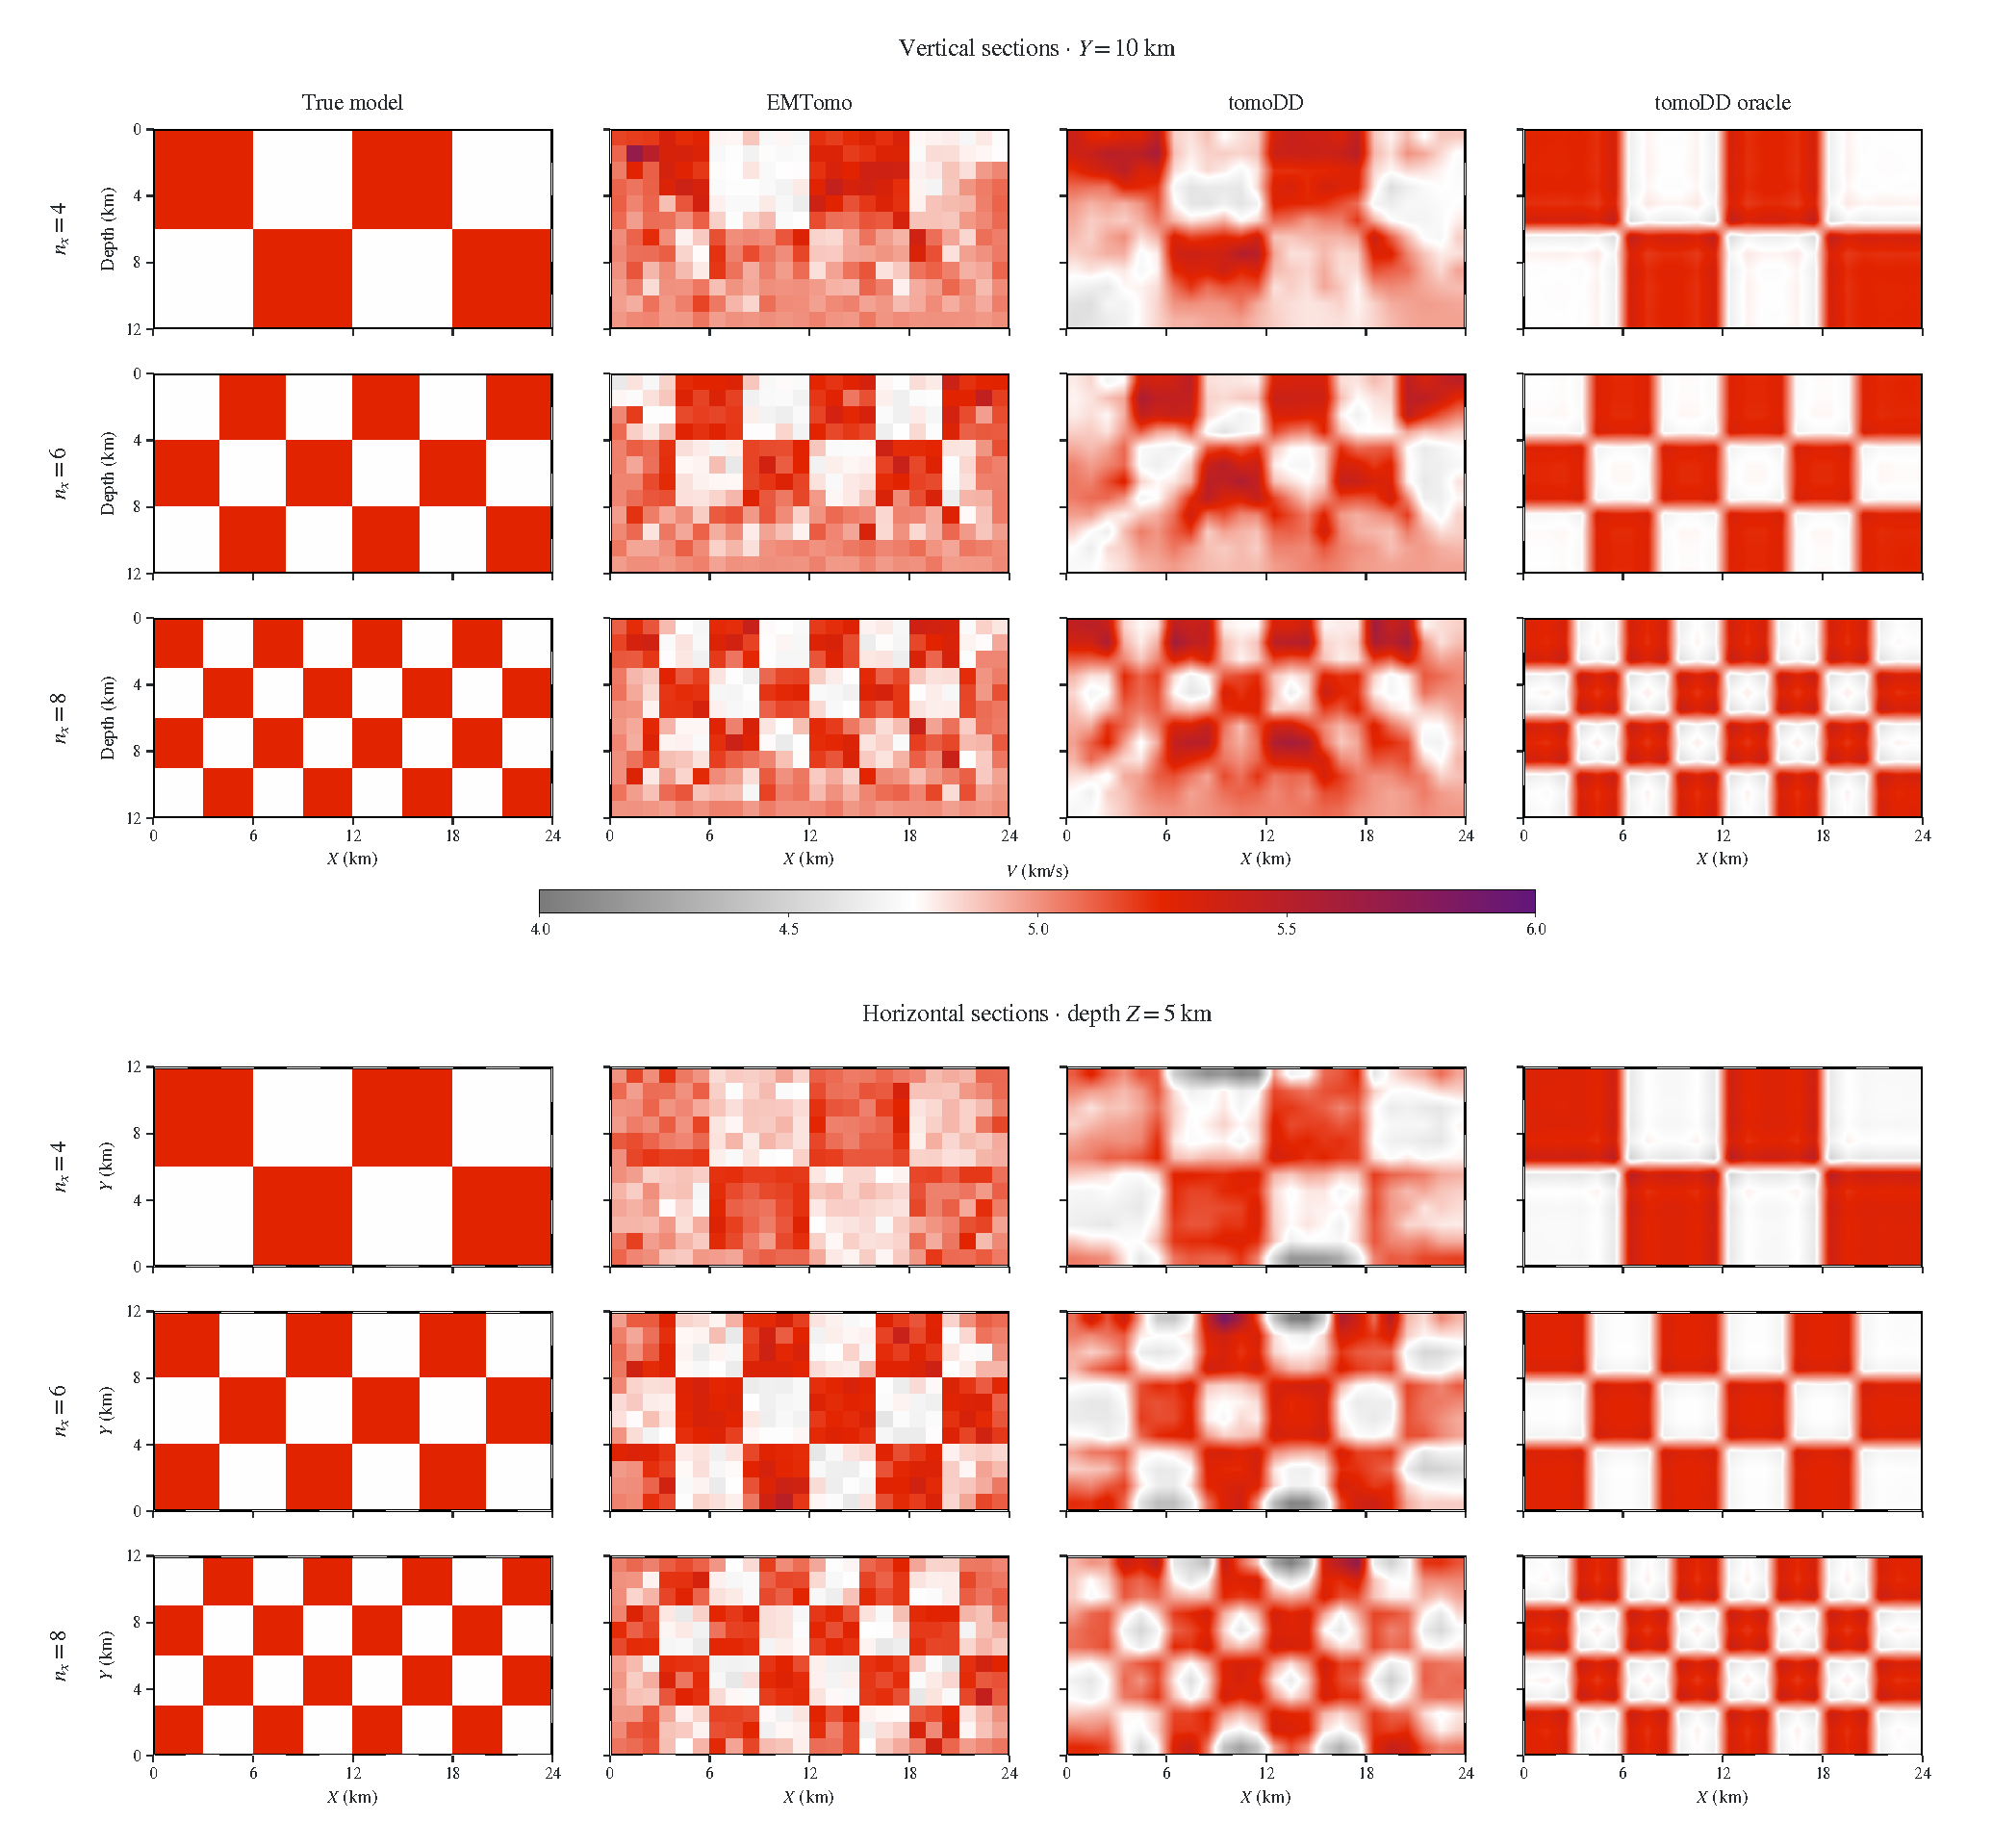
\includegraphics[width=\textwidth,height=0.62\textheight,keepaspectratio]{figures/checkerboard_nx4_nx6_nx8_comparison.pdf}
\begin{singlespace}
\caption{Checkerboard velocity reconstructions. Columns show truth, EMTomo after 12 updates, tomoDD after three iterations, and the trilinear representation oracle. The upper three rows are vertical sections at $Y=10$~km for $n_x=4,6,8$; the lower three are horizontal sections at $Z=5$~km in the same order. All panels share the velocity scale in km/s. The oracle is a truth-only representation reference, not an inversion result.}
\label{fig:checkerboard_comparison_current}
\end{singlespace}
\end{figure}
\FloatBarrier

Table~\ref{tab:checkerboard_locations} reports the 90th-percentile location error for each full catalog. Figure~\ref{fig:checkerboard_locations} shows the location estimates for the $n_x=6$ section, and Figure~\ref{fig:checkerboard_location_ecdf} shows the full-catalog error distributions.

\begin{table}[!htb]
\centering
\begin{singlespace}
\caption{Checkerboard hypocenter accuracy: 90th percentile of 3D location error (m), evaluated over all 1200 events. EMTomo locations precede the twelfth velocity update; tomoDD locations follow three joint iterations.}
\label{tab:checkerboard_locations}
\begin{tabular}{rrrr}
\toprule
$n_x$ & Cube side (km) & EMTomo & tomoDD \\
\midrule
4 & 6 & 505.9 & 599.2 \\
6 & 4 & 373.4 & 588.1 \\
8 & 3 & 402.5 & 609.1 \\
\bottomrule
\end{tabular}
\end{singlespace}
\end{table}

\begin{figure}[!htb]
\centering
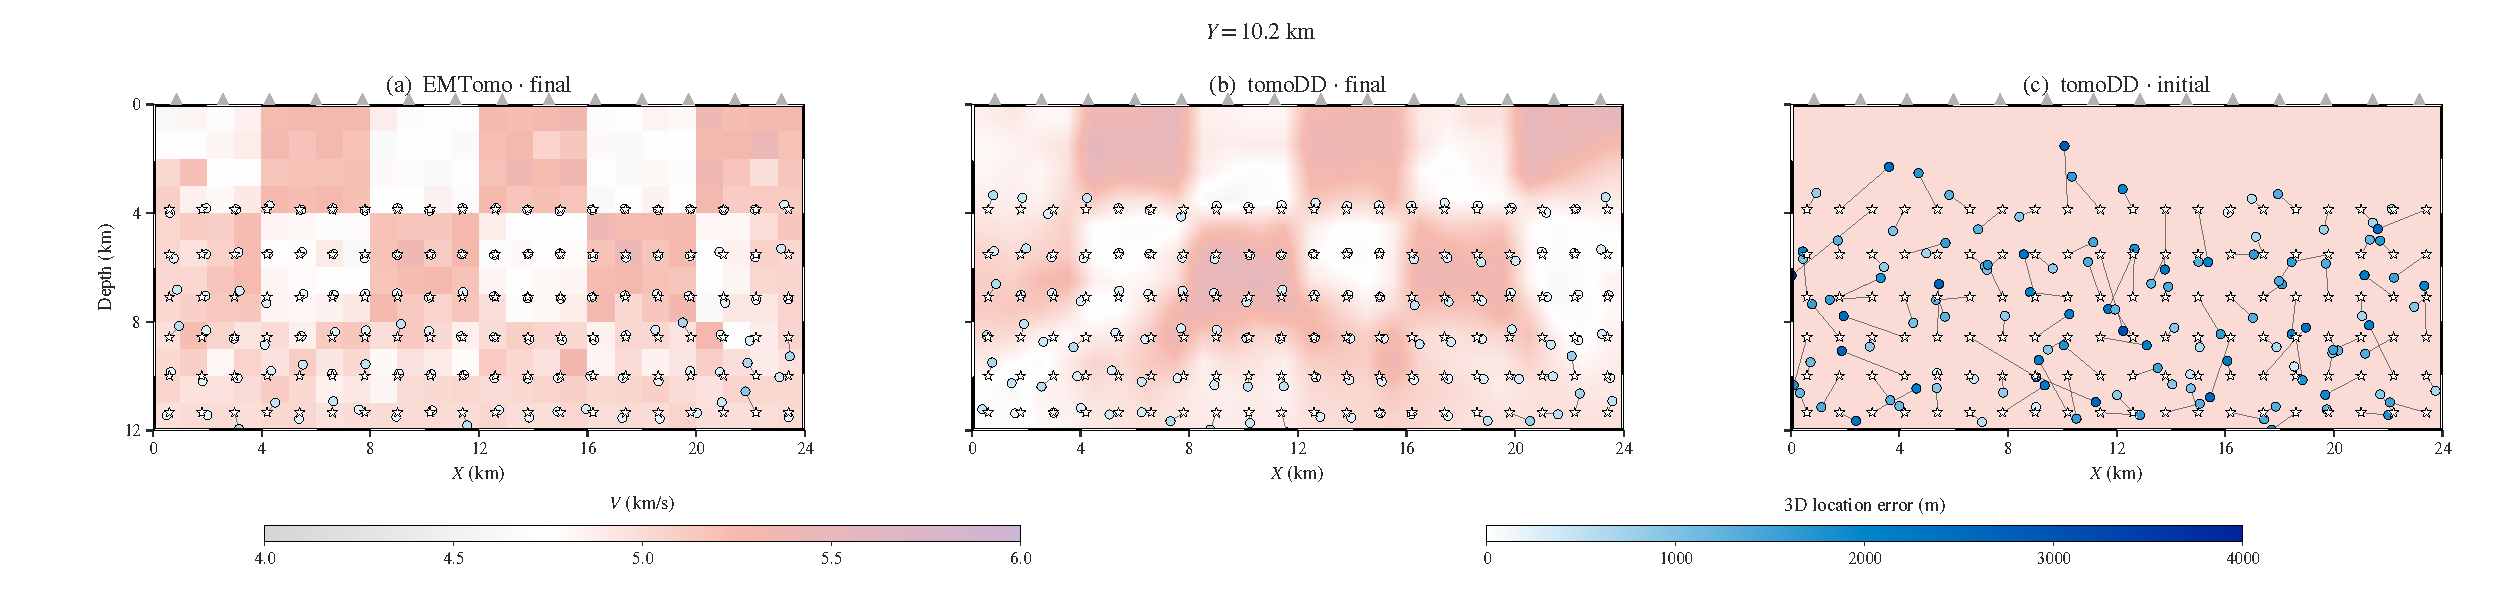
\includegraphics[width=\textwidth]{figures/checkerboard_nx6_locations_y10p2km.pdf}
\begin{singlespace}
\caption{Hypocenter estimates for the 120 events with true $Y=10.2$~km in the $n_x=6$ checkerboard: (a) EMTomo, (b) tomoDD, and (c) initial tomoDD locations. White stars mark true positions; circles mark estimates, connected to the truth by grey segments. Positions are projected onto the $X$--depth plane, while circle colors show full 3D location errors. Backgrounds show the corresponding final or initial velocity fields. EMTomo locations are from the E-step preceding the last velocity update.}
\label{fig:checkerboard_locations}
\end{singlespace}
\end{figure}

\begin{figure}[!htb]
\centering
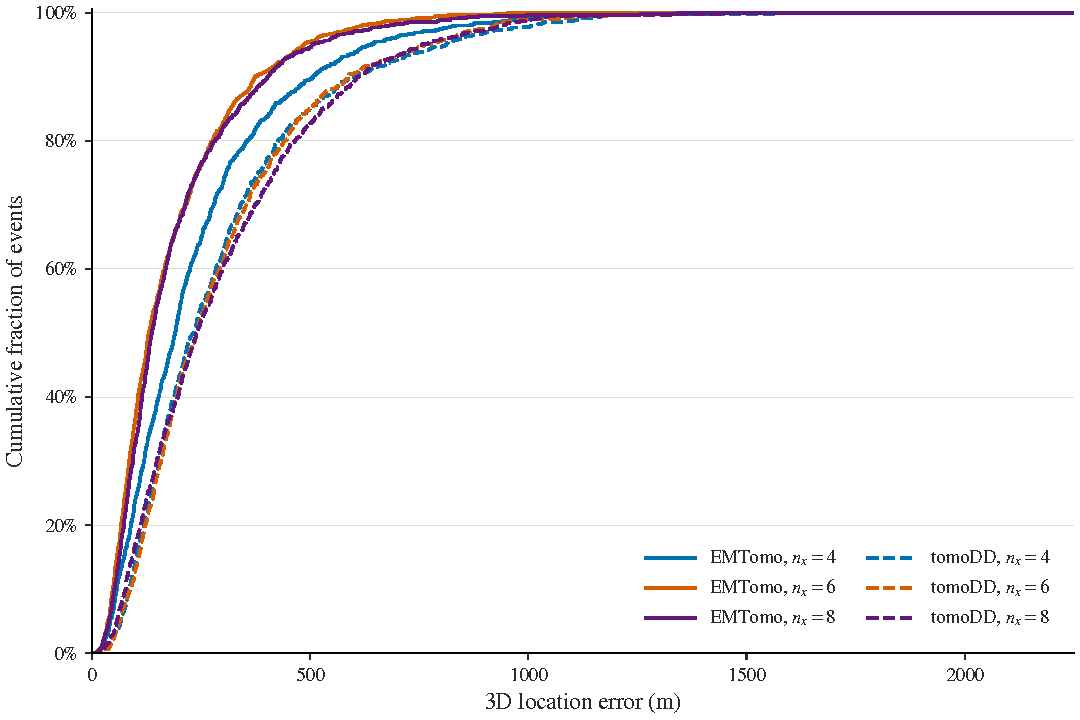
\includegraphics[width=0.85\textwidth]{figures/checkerboard_location_error_ecdf.pdf}
\begin{singlespace}
\caption{Cumulative distributions of 3D location error for all 1200 events in each checkerboard. Colors identify $n_x=4,6,8$; solid lines denote EMTomo and dashed lines tomoDD. EMTomo uses the E-step locations preceding the twelfth velocity update; tomoDD uses locations after three joint iterations. A higher curve indicates a larger fraction of events within a given error.}
\label{fig:checkerboard_location_ecdf}
\end{singlespace}
\end{figure}

\FloatBarrier
\subsection{Spherical anomalies}
\label{subsec:sphere_results}

Both experiments use the same $20\times7\times7$~km velocity model, sampled on 125-m cells (Figure~\ref{fig:spherical_anomalies_truth}). Four horizontal layers have velocities 3.8, 4.6, 5.2, and 5.7~km/s, with interfaces at depths 0.7, 1.9, and 3.4~km. Six spherical anomalies add signed velocity perturbations to this background. Each perturbation is constant inside half its radius and decreases to zero with a cosine taper between half-radius and the outer boundary. For spheres 1--6, the centers $(x,y,z)$ in km are $(3.5,2.5,1.2)$, $(8.0,4.8,2.0)$, $(12.5,2.4,2.6)$, $(16.5,4.5,1.6)$, $(6.0,2.2,3.6)$, and $(11.0,5.0,4.0)$; the corresponding radii are 0.9, 1.1, 1.2, 1.0, 1.1, and 1.0~km, and peak velocity increments are $+600$, $-650$, $+700$, $-600$, $+700$, and $-650$~m/s.

\begin{figure}[!htb]
\centering
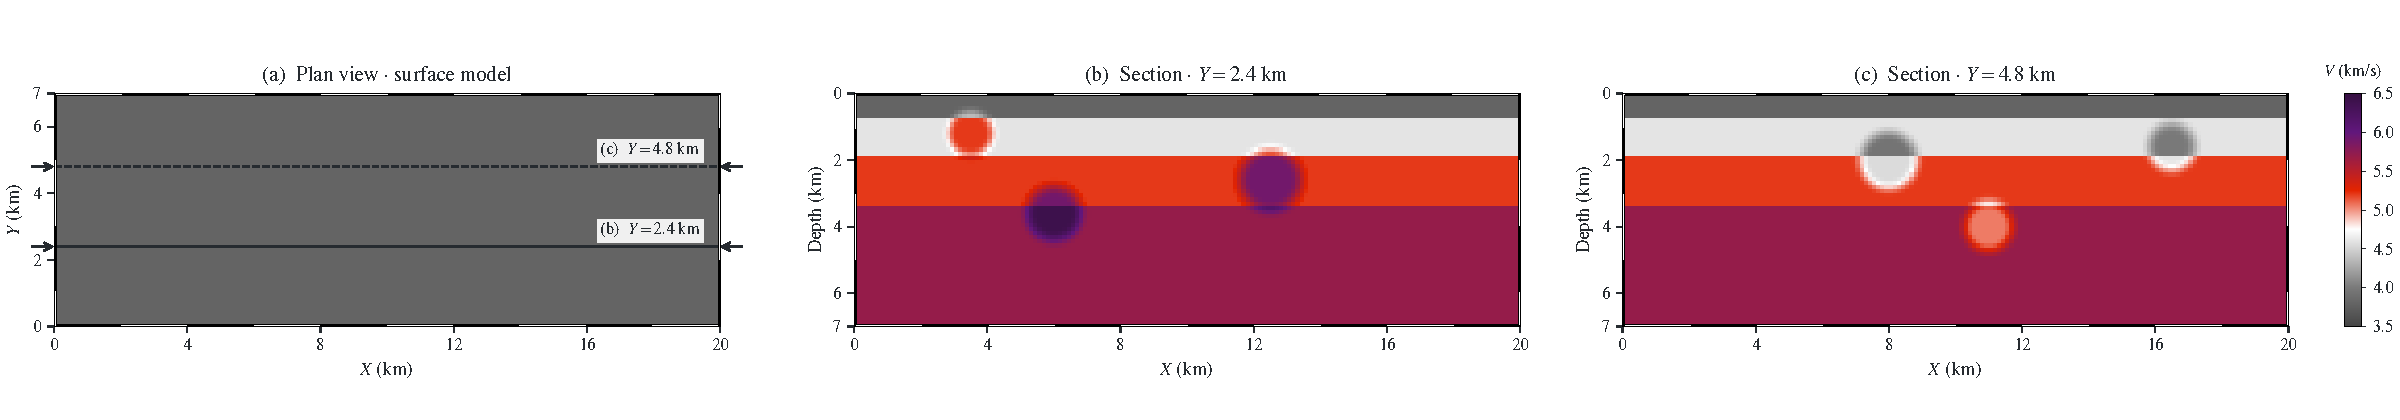
\includegraphics[width=\textwidth]{figures/spherical_anomalies_truth.pdf}
\begin{singlespace}
\caption{True velocity model shared by the artificial- and Geysers-geometry experiments. (a) Surface plan view with the two section lines. (b) Vertical section at $Y=2.4$~km, showing spheres 1, 3, and 5. (c) Vertical section at $Y=4.8$~km, showing spheres 2, 4, and 6. Both sections show the four-layer background and the native 125-m truth cells without added smoothing. All panels share the velocity scale in km/s; depth is positive downward.}
\label{fig:spherical_anomalies_truth}
\end{singlespace}
\end{figure}

The acquisition geometries are shown in Figure~\ref{fig:spherical_anomalies_geometry}. The artificial geometry contains 52 surface stations on a $13\times4$ grid and 1920 events on a $24\times8\times10$ lattice, with depths 0.75--5.25~km. The Geysers geometry uses 26 station positions and 3776 catalog event locations from 1--20 April 2011. The model top is at elevation 1166~m; station depths range from 0 to 839~m and event depths from 1.166 to 6.877~km. Station elevations and catalog depths are treated as sharing a vertical datum. Arrival times are synthetic in both experiments, with all event--station pairs observed: 99,840 and 98,176 P-wave picks, respectively. PyKonal uses a 62.5-m numerical grid. Before eventwise time referencing, noise is added with relative standard deviation 1\% and absolute standard deviation 0.01~s. All methods within each geometry use the same saved noisy picks.

\begin{figure}[!htb]
\centering
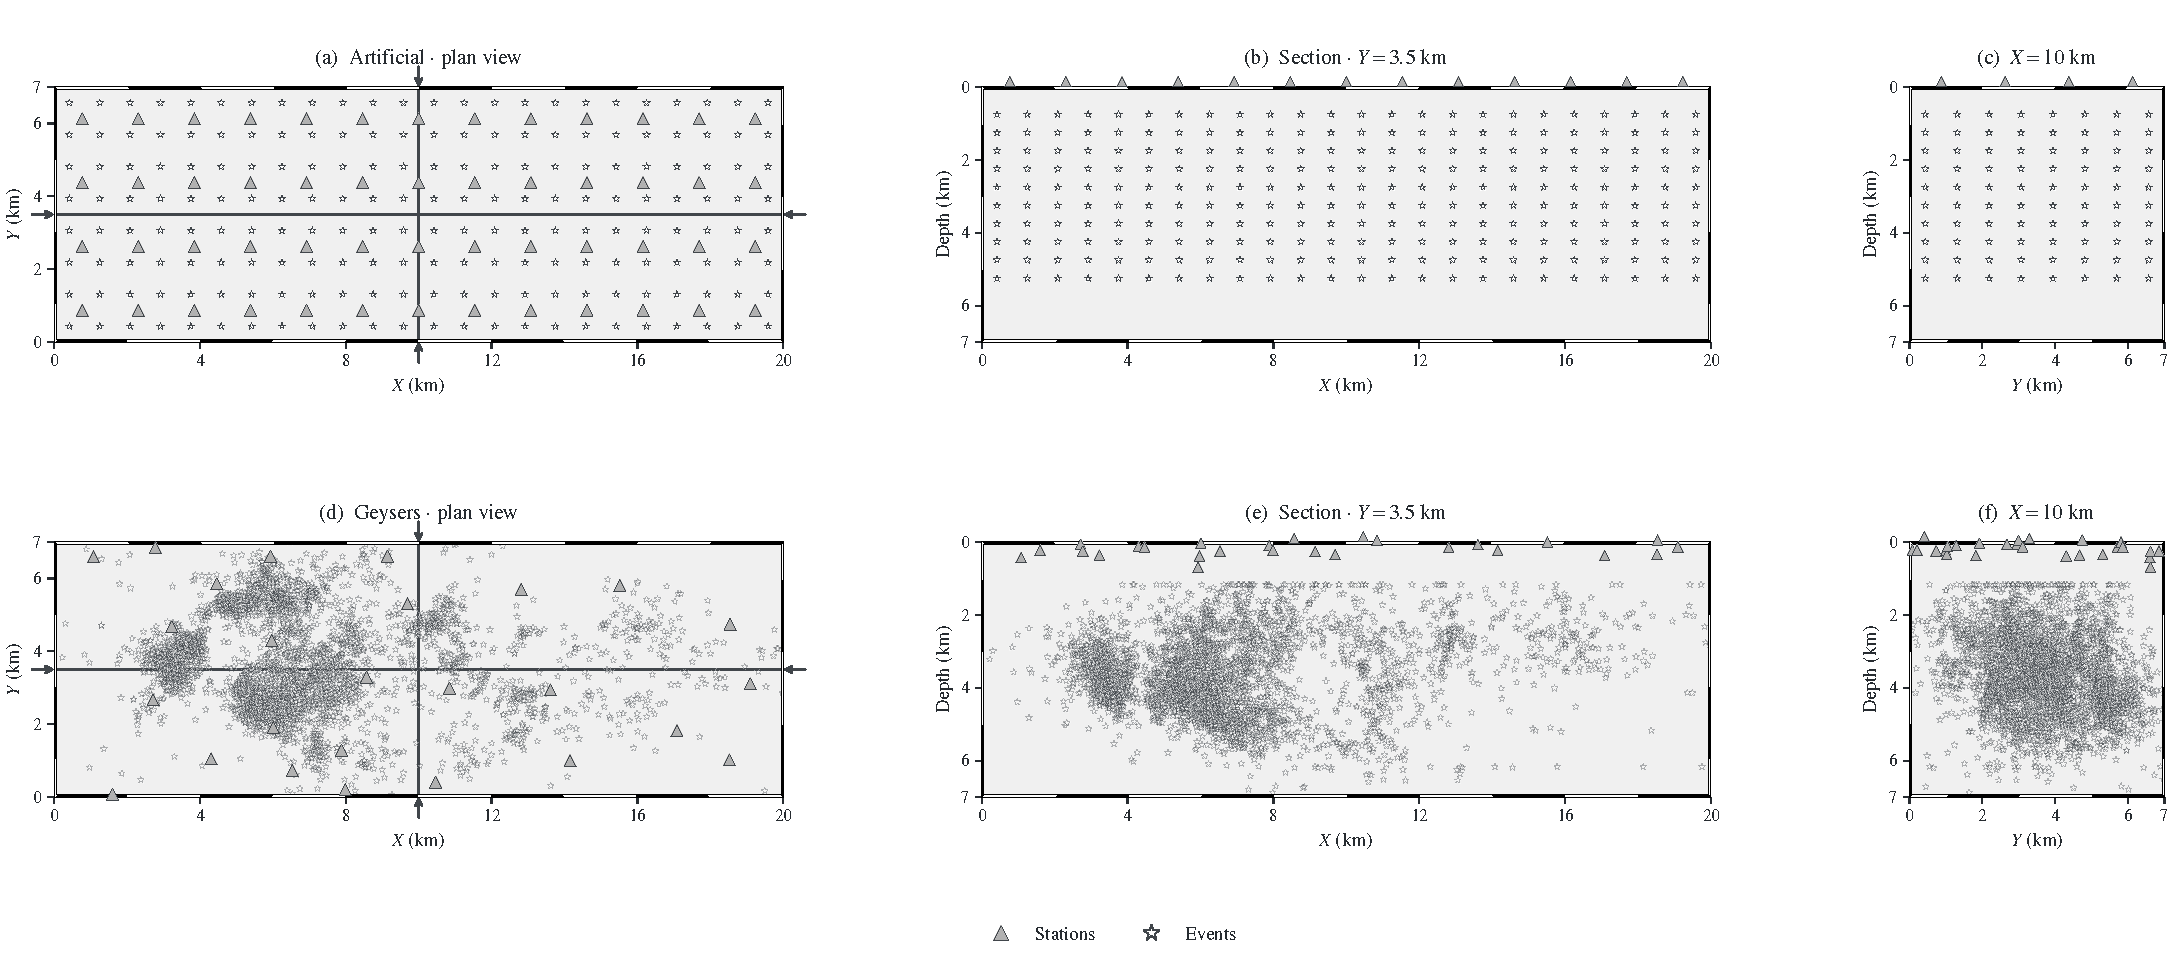
\includegraphics[width=\textwidth]{figures/spherical_anomalies_geometry.pdf}
\begin{singlespace}
\caption{Acquisition geometries for the spherical-anomaly experiments. The upper row shows the artificial geometry (52 stations, 1920 events); the lower row shows the Geysers geometry (26 stations, 3776 events). Columns show the plan view and perpendicular vertical projections onto $Y=3.5$~km and $X=10$~km, marked in the plan views. Grey triangles denote stations and white stars events. All coordinates are projected without spatial filtering; coincident projections are drawn once. The background is uniform, not a velocity field. Depth is positive downward, with station elevations retained as depths relative to the model top.}
\label{fig:spherical_anomalies_geometry}
\end{singlespace}
\end{figure}

EMTomo uses $20\times7\times7$ constant 1-km cells and a 125-m computational grid, with nearest-cell slowness evaluation. The initial velocity model contains the four background layers without spherical anomalies; no initial hypocenter catalog is supplied. Both hard and soft runs perform 12 updates and refine 15 candidate locations per event. Hard assignment retains one candidate, whereas soft assignment retains ten at temperature one. Candidate seeds are separated by at least one fine-grid cell in Chebyshev distance before continuous refinement. Both variants use $\lambda=1$, coverage-damping exponent two, coverage floor 0.05, reference coverage percentile 75, and a $\pm2\%$ cellwise velocity-step limit. The likelihood includes the specified pick-noise variance and an additional model-error standard deviation of 0.02~s.

TomoDD uses 980 free interior velocity nodes at the EMTomo cell centers, with 1-km spacing and fixed exterior nodes, giving a $22\times9\times9$ nodal grid. The initial interior velocity values match EMTomo's layered start; interpolation remains native to each method. Initial hypocenters are perturbed independently by a Gaussian standard deviation of 1~km per coordinate, with out-of-domain positions rejection-resampled. Event pairs are formed from this starting catalog using a 3-km distance cutoff and maximum degree four, yielding 3827 pairs for the artificial geometry and 7532 for Geysers. Differential times are computed from the same picks, giving 199,004 and 195,832 differential observations. TomoDD performs three joint velocity--hypocenter iterations with equal absolute and differential P-wave weights, damping 40, smoothing 5/5/5, and a 0.05-km ray-derivative step. These runs use the corrected horizontal regional boundary guard.

Figure~\ref{fig:spherical_anomalies_comparison} shows the reconstructions and their representation oracles. Table~\ref{tab:spherical_velocity} reports velocity RMSE over all 501,760 truth-cell centers and separately within each of the six anomaly supports. Table~\ref{tab:spherical_locations} reports the 90th-percentile 3D location error over each full catalog; the soft result uses the largest-weight hypothesis for each event.

\begin{figure}[!htb]
\centering
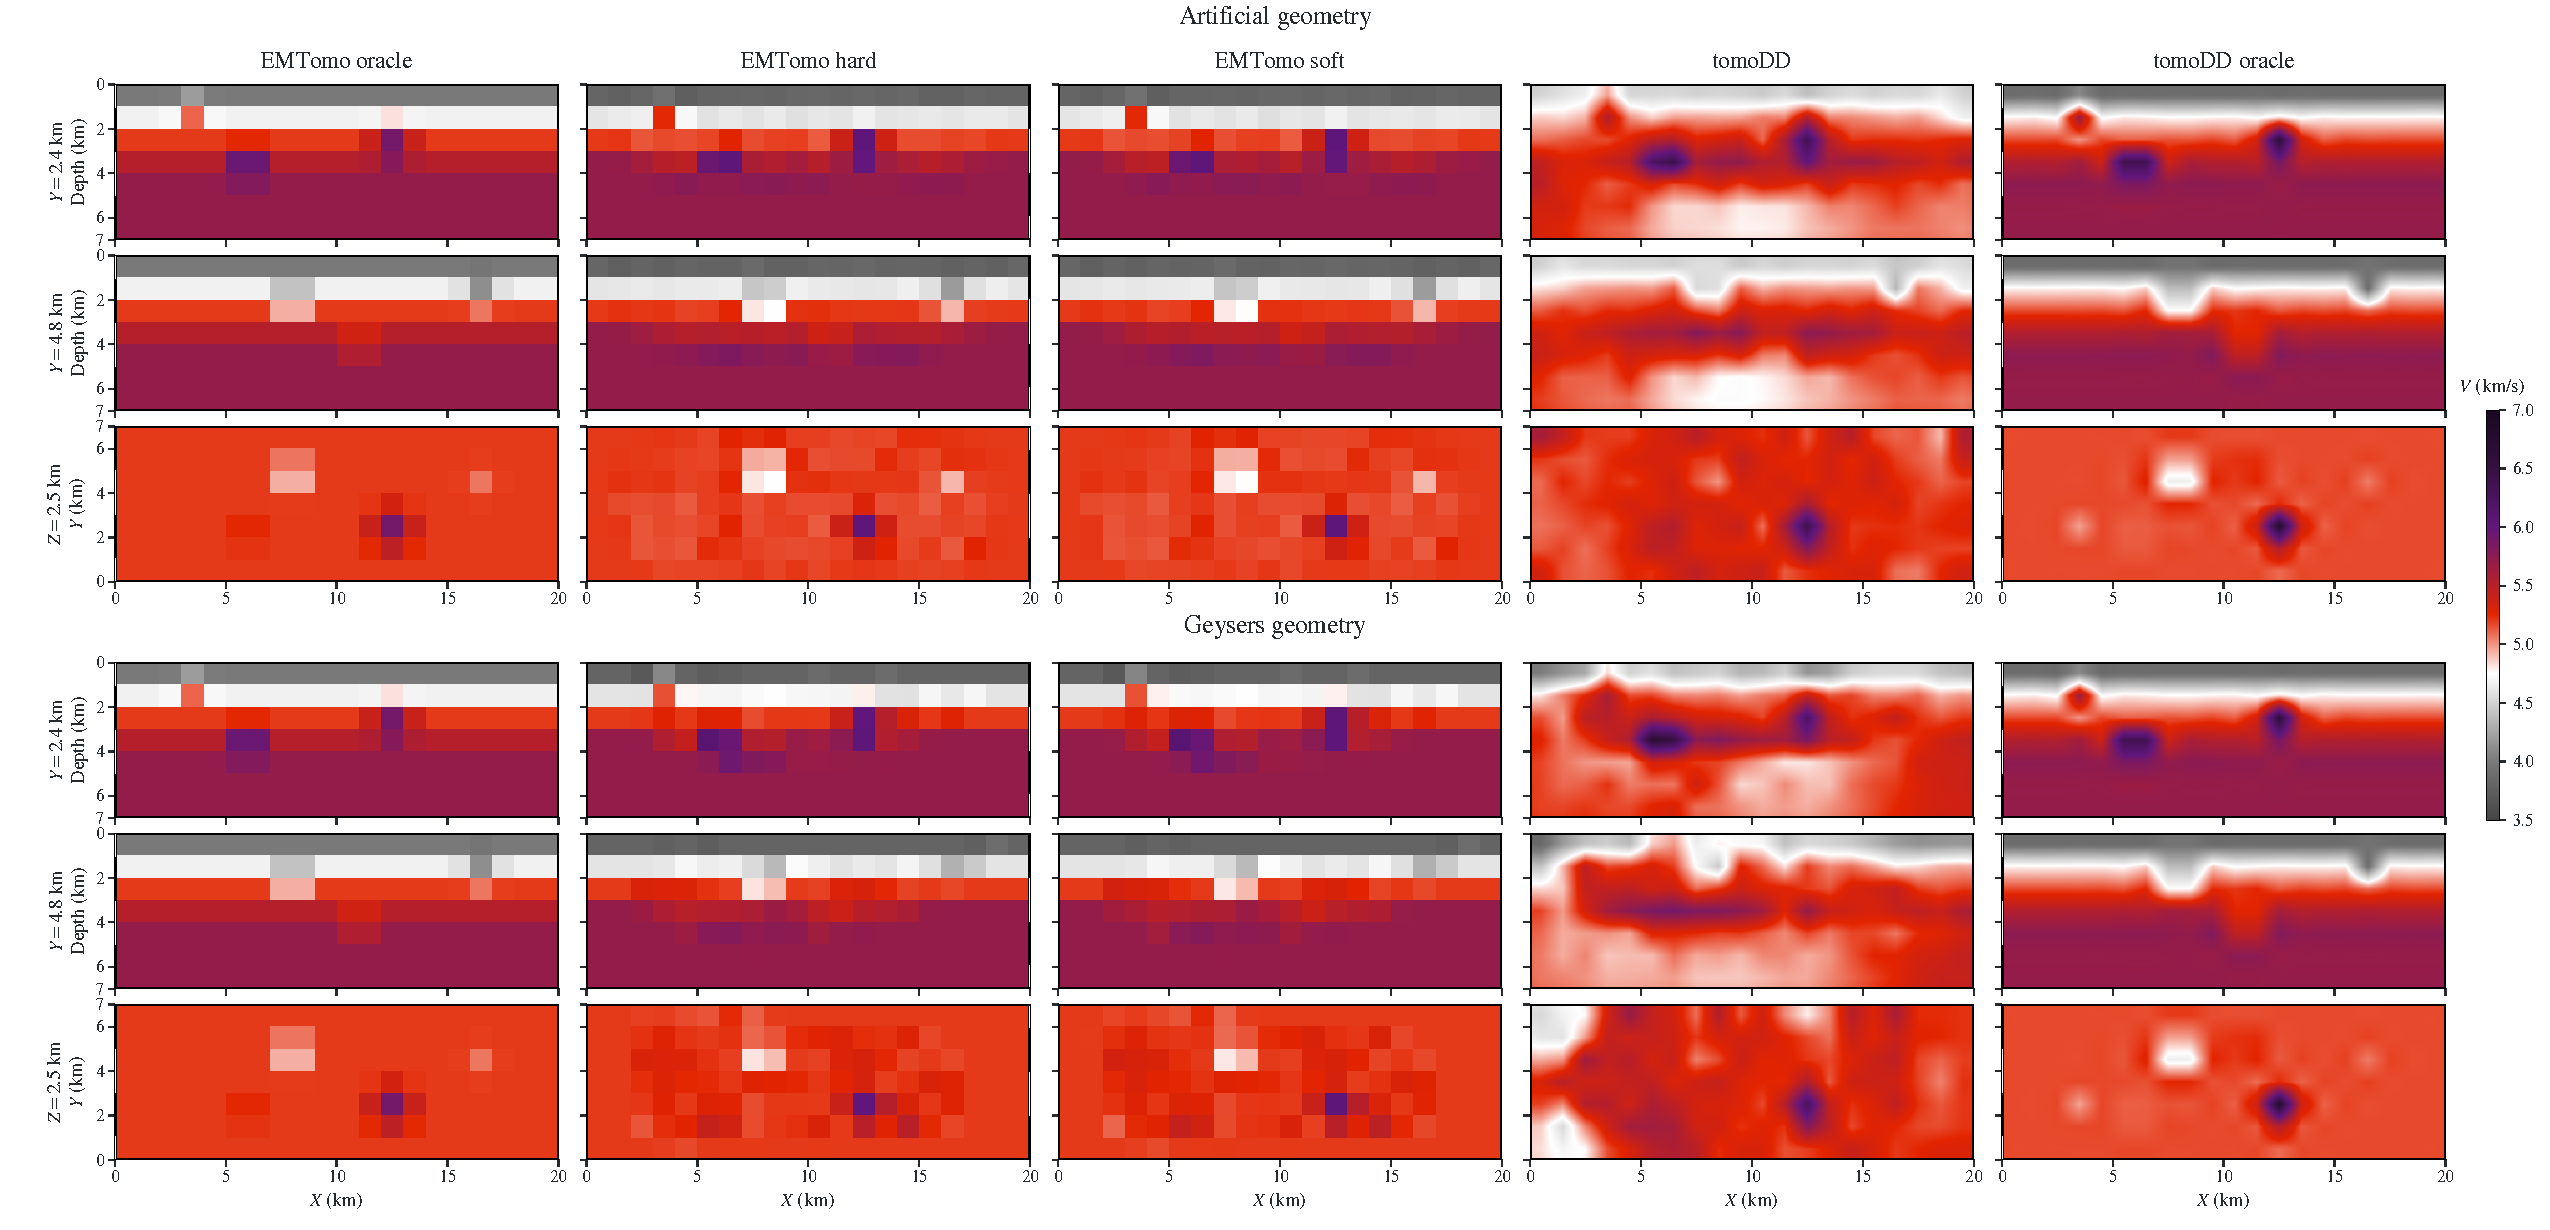
\includegraphics[width=\textwidth]{figures/spherical_anomalies_comparison.pdf}
\begin{singlespace}
\caption{Spherical-anomaly velocity reconstructions. Columns show the EMTomo constant-cell oracle, EMTomo hard and soft results after 12 updates, tomoDD after three joint iterations, and the tomoDD trilinear oracle. The upper and lower three rows show the artificial and Geysers geometries, respectively. Within each group, rows show vertical sections at $Y=2.4$ and $4.8$~km, as in Figure~\ref{fig:spherical_anomalies_truth}, followed by a horizontal section at $Z=2.5$~km. In horizontal sections, $Y$ increases upward. Oracles are truth-only representation references shared by both geometries. Fields retain their native constant-cell or trilinear representations, with no added smoothing. The shared vertical velocity scale is extended to 7~km/s to include all displayed values.}
\label{fig:spherical_anomalies_comparison}
\end{singlespace}
\end{figure}

\begin{table}[!htb]
\centering
\begin{singlespace}
\caption{Spherical-anomaly velocity RMSE (m/s), evaluated over the whole volume and within each anomaly's nonzero support. Sphere numbering follows the model specification in the text.}
\label{tab:spherical_velocity}
\small
\setlength{\tabcolsep}{4pt}
\begin{tabular}{lrrrrrrr}
\toprule
Method & Volume & Sphere 1 & Sphere 2 & Sphere 3 & Sphere 4 & Sphere 5 & Sphere 6 \\
\midrule
\multicolumn{8}{l}{Artificial geometry} \\
EMTomo hard & 203.3 & 480.1 & 282.4 & 307.2 & 311.5 & 342.2 & 317.5 \\
EMTomo soft & 203.2 & 478.9 & 282.4 & 308.2 & 311.5 & 342.2 & 316.9 \\
tomoDD & 506.4 & 447.0 & 361.6 & 288.5 & 379.3 & 387.7 & 353.1 \\
\midrule
\multicolumn{8}{l}{Geysers geometry} \\
EMTomo hard & 208.4 & 445.6 & 305.7 & 290.2 & 331.6 & 332.0 & 320.8 \\
EMTomo soft & 208.3 & 448.6 & 305.5 & 291.3 & 330.8 & 332.2 & 321.7 \\
tomoDD & 501.0 & 475.1 & 404.1 & 266.0 & 507.0 & 391.0 & 341.1 \\
\bottomrule
\end{tabular}
\end{singlespace}
\end{table}

\begin{table}[!htb]
\centering
\begin{singlespace}
\caption{Spherical-anomaly hypocenter accuracy: 90th percentile of 3D location error (m). EMTomo locations are from the E-step preceding the twelfth velocity update; tomoDD locations follow three joint iterations.}
\label{tab:spherical_locations}
\begin{tabular}{lrrr}
\toprule
Geometry & EMTomo hard & EMTomo soft & tomoDD \\
\midrule
Artificial & 231.2 & 231.5 & 445.8 \\
Geysers & 223.5 & 213.5 & 961.9 \\
\bottomrule
\end{tabular}
\end{singlespace}
\end{table}
\FloatBarrier

\subsection{Real data}
\label{subsec:geysers_results}

\section{Discussion}
\label{sec:discussion}

In the checkerboard test, both methods recover the alternating pattern most clearly in the horizontal sections, while recovery deteriorates at depth (Figure~\ref{fig:checkerboard_comparison_current}). EMTomo retains sharp cell boundaries but shows local variability; tomoDD produces smoother transitions. The trilinear oracle also rounds the true block boundaries, illustrating the contribution of the velocity representation to these differences. Its increasing RMSE as cube size decreases reflects this representational limitation, whereas the aligned EMTomo cells represent the checkerboard truth exactly.

For these runs, EMTomo has lower whole-volume velocity RMSE and lower 90th-percentile location error than tomoDD at all three cube sizes (Tables~\ref{tab:checkerboard_velocity} and~\ref{tab:checkerboard_locations}). The location comparison for $n_x=6$ shows that both methods place events close to their true positions, despite the perturbed starting catalog supplied to tomoDD (Figure~\ref{fig:checkerboard_locations}). These results compare the stated workflows: the methods differ in velocity representation, regularization, and iteration count, so the differences cannot be attributed solely to their treatment of hypocenters.
